
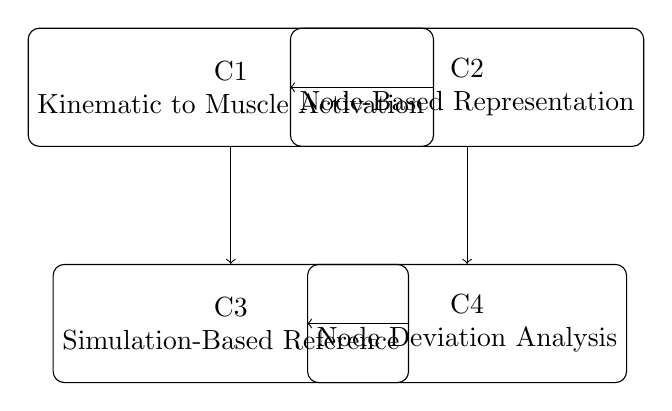
\begin{tikzpicture}[
node distance=3cm,
box/.style={draw, rounded corners, minimum width=4cm, minimum height=1.5cm, align=center}
]

\node[box] (c1) {C1\\Kinematic to Muscle Activation};
\node[box, right of=c1] (c2) {C2\\Node-Based Representation};
\node[box, below of=c1] (c3) {C3\\Simulation-Based Reference};
\node[box, right of=c3] (c4) {C4\\Node Deviation Analysis};

\draw[->] (c1) -- (c2);
\draw[->] (c1) -- (c3);
\draw[->] (c2) -- (c4);
\draw[->] (c3) -- (c4);

\end{tikzpicture}
